\documentclass{article}
\usepackage{cite}

\usepackage{graphicx}
\begin{document}
\begin{figure}[!tbp]
  \caption{Top Pay-Level Domains (PLDs) of entities in BTC-2009}
  \centering
  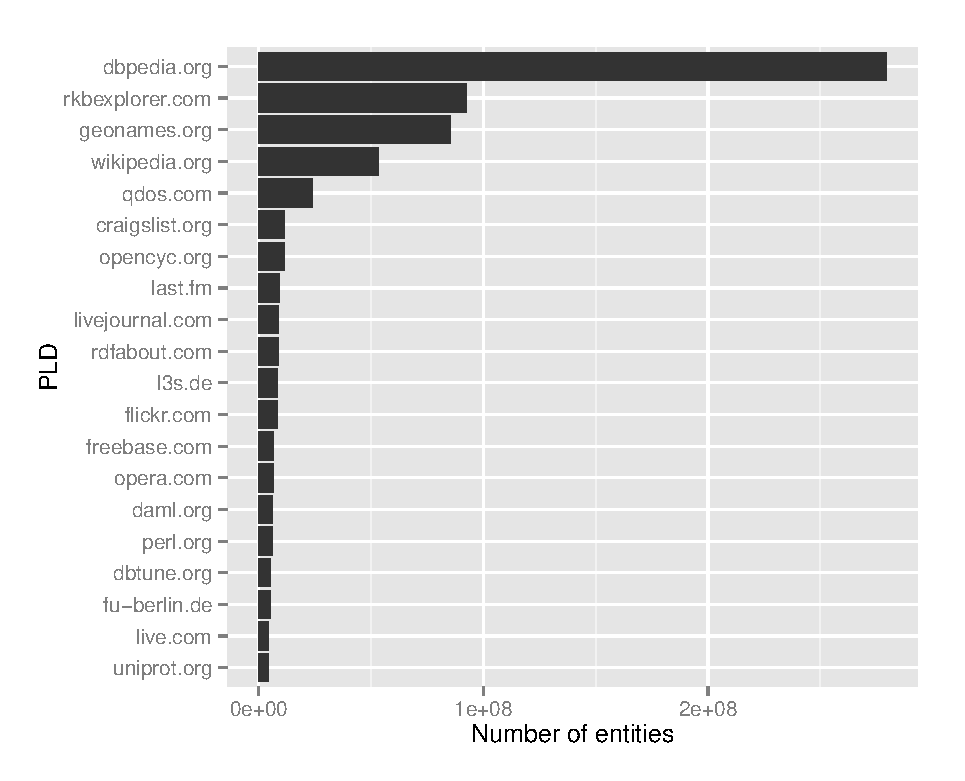
\includegraphics[width=0.7\textwidth]{../btc-2009}
  \label{fig:btc2009}
\end{figure}
\begin{figure}[!tbp]
  \caption{Top Pay-Level Domains (PLDs) of relevant entities in Semantic Search
    Challenge 2010/2011}
  \centering
  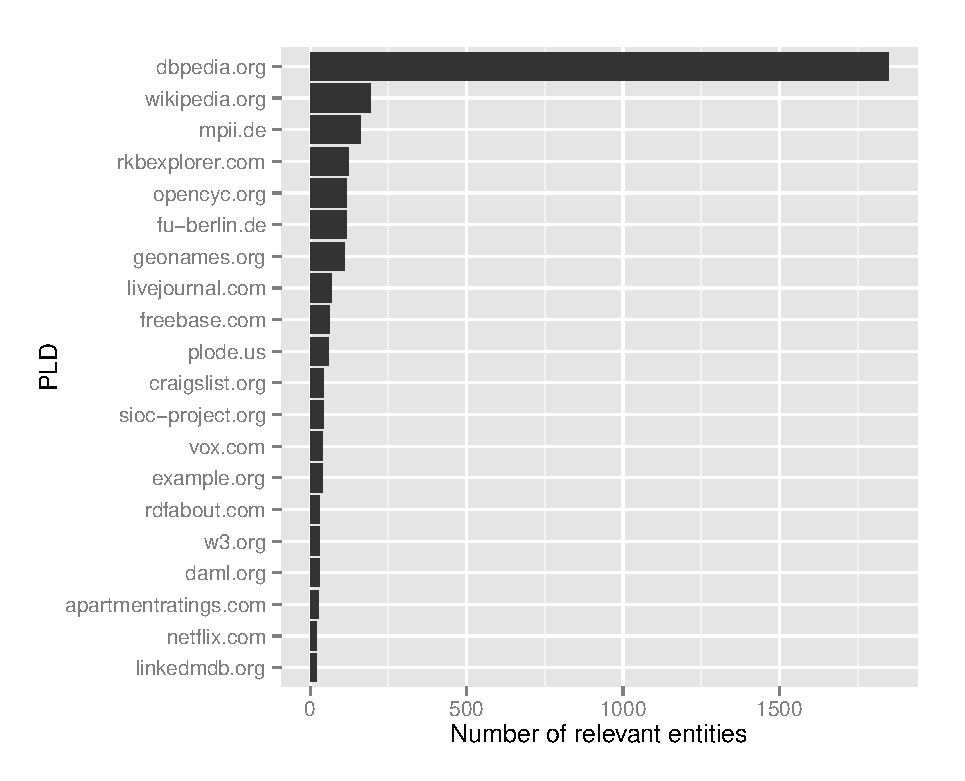
\includegraphics[width=0.7\textwidth]{../relevant}
  \label{fig:relevant}
\end{figure}

Figures~\ref{fig:btc2009} and~\ref{fig:relevant} show numbers of entities for
Top-20 Pay-Level Domains for the whole BTC-2009 dataset and relevant results
from SemSearch Challenge judgments only respectively. It can be observed that in
BTC-2009 dataset entities are significantly skewed towards DBpedia, and for
SemSearch Challenge this disproportion is even higher as was noted in
\cite{balog2013test}. Speaking of numbers, in the whole BTC-2009 dataset
DBpedia entities constitute $34.6\%$ of all entities and in relevance judgments
they constitute $48.9\%$ of all relevant results.

% Starting from BTC-2012 \cite{btc-2012} the problem was mostly solved as can be
% seen in \cite{btc-2012-stats}

\bibliography{desc}{}
\bibliographystyle{plain}
\end{document}